{\bfseries ДОЛЖНА БЫТЬ СТАТЬЯ ЖАМАНГАРИНА С.}

{\bfseries ҒТАХР 65.55.37}

\section{ХОЛЕКАЛЬЦИФЕРОЛДЫҢ ОЛИГОҚАНТПЕН СУДА ЕРИТІН КЕШЕНІН АЛУ}

\begin{center}
{\bfseries С. Фазылов\textsuperscript{1*}, O.Нүркенов\textsuperscript{1},
A. Искинеева\textsuperscript{2}, A.Мұстафаева\textsuperscript{2},}

{\bfseries И. Пустолайкина\textsuperscript{3}, А.
Сарсенбекова\textsuperscript{3}, А.Свидерский\textsuperscript{4}}

\textsuperscript{1}Органикалық синтез және көмірхимиясы институты,
Қарағанды, Қазақстан,

\textsuperscript{2}С.Сейфуллин атындағы Қазақ агротехникалық
университеті, Астана, Қазақстан,

\textsuperscript{3} Е.Бөкетов атындағы Қарағанды университеті,
Қарағанды, Қазақстан,

\textsuperscript{4}Инновациялық Еуразия университеті, Павлодар,
Қазақстан,

e-mail: \href{mailto:iosu8990@mail.ru}{\ul{iosu8990@mail.ru}}
\end{center}

Мақалада майда еритін холекальциферолдың крахмал олигоқантымен капталған
түрін алу бойынша зерттеу нәтижелері келтірілген. Өндіріс жағдайында
ылғалды ортада майда еритін холекальциферолдың жоғары липофильділігі
және төмен ерігіштігі белгілі бір қиындықтар тудырады. Осы себепті
биофармацевтикалық және қоректік қасиеттері жақсартылған холекальциферол
дәруменінің (ХД) суда еритін түрлерін алудың технологиялық әдістерін
жасау қажеттілігі туындайды. Жүргізілген зерттеулер нәтижесінде ХД
крахмалдың олигоқантымен (бета-тұйықдекстрин, β-ТД) қапталған суда
еритін кешені алынды. Молекулалық үлгілеудің \emph{in silico}
әдістерімен ХД-дың β-ТД-мен кешендерінің клатратты түрлерінің түзілу
механизмдері зерттелді. Клатрат түзілуіндегі кристаллдың беткі қабатының
морфологиясы электронды микроскоп деректерімен әртүрлі үлкейту
жағдайында сарапталды. Термографиялық өлшеулердің нәтижелері, сондай-ақ
бастапқы және соңғы қосылыстардың салыстырмалы \textsuperscript{1}Н және
\textsuperscript{13}С ЯМР спектроскопиялық параметрлері ұсынылды.
Алынған жаңа ғылыми нәтижелер олигоқанттың гидрофобты қуысында ішкі
(инклюзивті) кешен пайда болады деген қорытынды жасауға мүмкіндік
береді.

{\bfseries Түйін сөздер:} холекальциферол, функционалды тамақтану,
олигоқанттар, β-тұйықдекстрин, қосылу кешендері, клатрат

\begin{center}
{\large\bfseries ПОЛУЧЕНИЕ ВОДОРАСТВОРИМОГО КОМПЛЕКСА ХОЛЕКАЛЬЦИФЕРОЛА С
ОЛИГОСАХАРИДОМ}

{\bfseries С. Фазылов\textsuperscript{1*}, O.Нуркенов\textsuperscript{1},
A. Искинеева\textsuperscript{2}, \textsuperscript{2}A.
Мустафаева\textsuperscript{2},}

{\bfseries И. Пустолайкина\textsuperscript{3},
А.Сарсенбекова\textsuperscript{3}, А.Свидерский\textsuperscript{4}}

\textsuperscript{1}Институт органического синтеза и углехимии РК,
Караганда, Казахстан,

\textsuperscript{2} Казахский агротехнический университет имени С.
Сейфуллина, Астана, Казахстан,

\textsuperscript{3} Карагандинский университет имени Е.Букетова,
Караганда, Казахстан,

\textsuperscript{4}Инновационный Евразийский университет, Павлодар,
Казахстан,

e-mail: iosu8990@mail.ru
\end{center}

В статье представлены результаты исследования по получению
капсулированной формы жирорастворимого холекальциферола с олигосахаридом
крахмала. В производственных условиях высокая липофильность и низкая
растворимость нативной формы холекальциферола в водной среде создает
определенные трудности. По этой причине возникает необходимость
разработки технологических способов получения водорастворимых форм
витамина холекальциферола (ХД) с улучшенными биофармацевтическими и
питательными свойствами. В результате выполненных исследований получен
водорастворимый комплекс клатратного типа холекальциферола с
бета-олигосахаридом крахмала (бета-циклодекстрином, β-ТД). Методами
молекулярного моделирования выполнено \emph{in silico} изучение
механизмов образования комплексов включения ХД с β-ТД- ном. Морфологии
поверхности кристаллов при клатратообразовании оценены данными
электронного микроскопа при различных увеличениях. Представлены
результаты термографических измерений, а также сравнительные
\textsuperscript{1}Н и \textsuperscript{13}С ЯМР-спектроскопические
параметры исходных и конечных соединений. Полученные новые научные
результаты позволяют сделать вывод, что в гидрофобной полости
олигосахарида образуется внутренний (инклюзивный) комплекс.

{\bfseries Ключевые слова:} холекальциферол, функциональное питание,
олигосахариды, β-циклодекстрин, клатрат.

\begin{center}
{\large\bfseries PREPARATION OF A WATER-SOLUBLE COMPLEX OF CHOLECALCIFEROL WITH
AN OLIGOSACCHARIDE}

{\bfseries S. Fazylov\textsuperscript{1*}, O. Nurkenov\textsuperscript{1},
A. Iskineyeva\textsuperscript{2}, A. Mustafayeva\textsuperscript{2},}

{\bfseries I. Pustolaikina\textsuperscript{3},
A.Sarsenbekova\textsuperscript{3}, A.Sviderskiy\textsuperscript{4}}

\textsuperscript{1}Institute of Organic Synthesis and Coal Chemistry,
Karaganda, 100008, Kazakhstan,

\textsuperscript{2} Kazakh Agrotechnical University, named after S.
Seifullin, Astana, 010000, Kazakhstan,

\textsuperscript{3} Karagandа University named after E.Buketov,
Karaganda, 100024, Kazakhstan,

\textsuperscript{4}Innovativ Eurasian University, Pavlodar, 140000,
Kazakhstan)

e-mail: \href{mailto:iosu8990@mail.ru}{\ul{iosu8990@mail.ru}}
\end{center}

The article presents the results of a study on the preparation of a
encapsulated form of fat-soluble cholecalciferol with starch
oligosaccharide. In production conditions, the high lipophilicity and
low solubility of the native form of cholecalciferol in an aqueous
medium creates certain difficulties. For this reason, there is a need to
develop technological methods for obtaining water-soluble forms of
vitamin cholecalciferol with improved biopharmaceutical and nutritional
properties. As a result of the performed studies, a water-soluble of
cholecalciferol inclusion complex with β-cyclodextrin (β-CD) was
obtained. Molecular modeling methods were used to study in silico the
mechanisms of formation of cholecalciferol inclusion complexes with
β-CD. The morphologies of the crystal surface during clathrate formation
are estimated by electron microscope data at various magnifications. The
results of thermographic measurements, as well as comparative
\textsuperscript{1}H and \textsuperscript{13}C NMR spectroscopic
parameters of the initial and final compounds are presented. The
obtained new scientific results allow us to conclude that an internal
(inclusive) complex is formed in the hydrophobic cavity of the
oligosaccharide.

{\bfseries Keywords:} cholecalciferol, functional food, oligosaccharide,
β-cyclodextrin, inclusion complexes, clathrate.

\begin{multicols}{2}
{\bfseries Кіріспе} Бүгінгі таңда, қолда бар соңғы медициналық деректерге
сәйкес, бүкіл әлем бойынша халықтың көпшілігі холекальциферол
дәруменінің (ХД) жетіспеушілігіне тап болуда. Қазіргі уақытта ХД
тапшылығы пандемия деп танылды {[}1,2{]}. ХД-нің адам ағзасындағы
кальций мен фосфордың метаболизміне қатысады. Бұл витамин сүйектердің,
эндокриндік {[}1{]} және адам ағзасының басқа жүйелерінің денсаулығын
қалыптастыру және сақтау үшін қажет. Соңғы зерттеулер ХД-тің қатерлі
ісік {[}3{]}, жүрек-қан тамырлары аурулары, қант диабеті және басқа
аурулардың алдын алудағы рөлін нақтылады {[}4-6{]}. Миллиондаған мектеп
жасына дейінгі балалар ХД тапшылығын анықтайды {[}1{]}. Азық-түлік ХД
қажеттіліктерін толығымен қамтымайды. Мұндай жағдайларда тамақты
дәрименмен қосымша байыту қажет. ХД молекуласында олефиндік байланыстар
көп, сондықтан температура, оттегі және жарық сияқты қоршаған орта
әсерлері жағдайларына байланысты тағамды өңдеу және сақтау кезінде оңай
тотығады. Өндіріс жағдайында су

ортасындағы ХД қалыпты түрінің липофильділігі мен суда төмен ерігіштігі
(1 мг/100 мл-ден аз) белгілі бір қиындықтар тудырады. Осы себепті
биофармацевтикалық және тағамдық қасиеттері жақсартылған
ДД\textsubscript{3} дәруменінің суда еритін түрлерін алудың
технологиялық әдістерін жасау қажеттілігі туындайды. Бұл жұмыста біз
крахмалдың 7 глюкозидті қалдығынан тұратын β-тұйықдекстринмен (β-ТД)
холекальциферолды қаптау нәтижелерін зерттедік. ХД молекуласының майлы
ерітіндісін қолдану арқылы осы ХД молекулаларының β-ТЦ молекулаларының
цилиндрлік гидрофобты қуыстарына енгізу арқылы, "қонақ-қожайын"
кешенінің түзілуін іске асырдық (сурет1).
\end{multicols}

\begin{figure}[H]
  \centering
  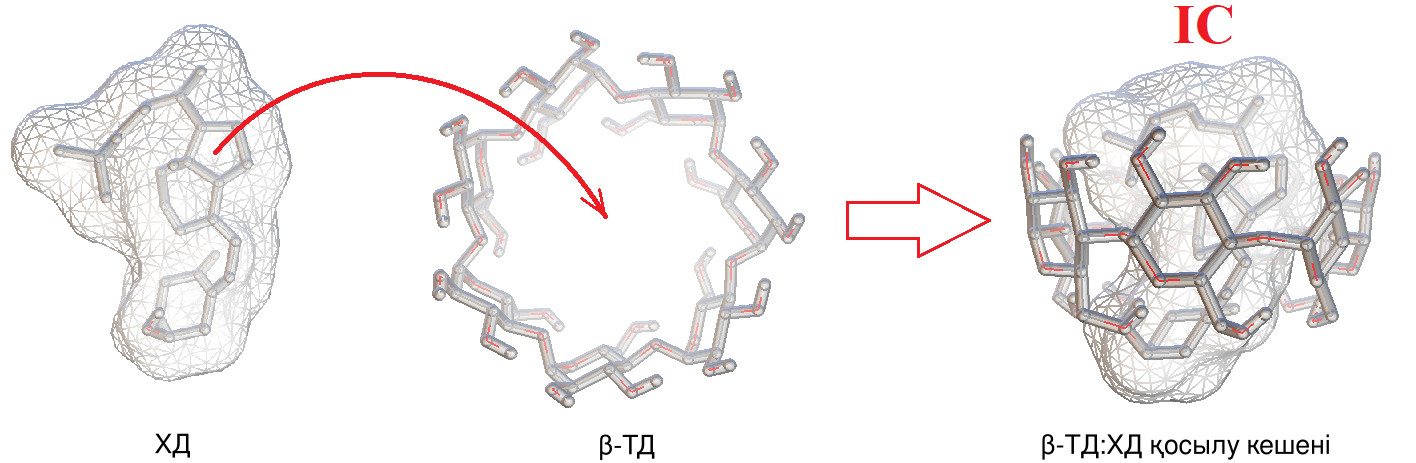
\includegraphics[width=0.8\textwidth]{image22}
  \caption*{Сурет 1 - Холекальциферолдың β-ТД-мен қосылу кешенінің қалыптасуының схемалық көрінісі}
\end{figure}

\begin{multicols}{2}
ХД тотықтырғыштардың әсерінен майлы қабық ішінде жақсы сақталады және
биожетімділігі жақсы болады {[}7{]}. Сондықтан ХД -ды β-ТД-мен кешенге
қосу табиғатын түсіну өте маңызды. Осы жұмыста біз β-ТД:ХД қосылу
кешенін микротолқынды әдіспен алдық {[}8{]}. Алынған кешен ИК-Фурье,
\textsuperscript{1}H және \textsuperscript{13}C ЯМР спектроскопиясы,
СEM, ДTГ әдістемелерімен зерттелді.

{\bfseries Материалдар мен әдістемелер.} Жұмыста келесі реагенттер
қолданылды: олигосахарид β-тұйықдекстрин (β-ТД, Fluka фирмасынан сатып
алынған, 99,5\%), ХД (250 мкг (10.000 ХБ),
С\textsubscript{27}Н\textsubscript{44}О, (Олдрич компаниясы). ЯМР
\textsuperscript{1}Н, \textsuperscript{13}С барлық өлшемдері
DMSO-d\textsubscript{6} (Олдрич) ерітінділерінде жүргізілді, басқа
химиялық заттар реагенттер класының аналитикалық тазалығында болды.
(ХД)-нін тұйықдекстриндермен молекулалық докингтеу autodock 4.2.6,
MGLTools 1.5.7 {[}9{]} және AutoDock 4.2.6-да енгізілген ламарков
генетикалық алгоритмі (LGA) {[}10{]} бағдарламалары арқылы жүзеге
асырылды. Жартылай иілгіш қондыру әдісі қолданылды, онда рецептор қатты
зат ретінде қарастырылды, ал лиганд белгілі бір текше аймақта айналды
және қозғалыста болды. Байланыс энергиясы ретінде \emph{AutoDock}
электростатикалық, гидрофобты және сольвациялық әсерлерді, сондай-ақ
конфигурация энтропиясын қоса алғанда, еркін байланыс энергиясына
негізделген эмпирикалық бағалау функциясын пайдаланды. \emph{Autodock}
тәсілі торға негізделген молекулалық жақындық потенциалдарын қолдана
және энергияны жылдам бағалай отырып, Монте-Карлоның модельді үйлестіру
әдісін қолданады. Химиялық құрылымдар PubChem Substance and Compound
дерекқорынан алынды (pubchem.ncbi.nlm.nih.gov) {[}10{]}. Химиялық
құрылымның бірегей идентификаторлары ретінде 444041 (циклодекстрин),
5280795 (холекальциферол) алынды (сурет 2).
\end{multicols}

\begin{figure}[H]
  \centering
  \begin{subfigure}[b]{0.4\textwidth}
    \centering
    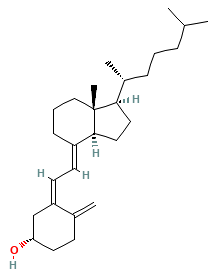
\includegraphics[height=\textwidth]{image23}
    \caption*{(a) Cholecalciferol (ДД\textsubscript{3})}
  \end{subfigure}
  \hfill
  \begin{subfigure}[b]{0.4\textwidth}
    \centering
    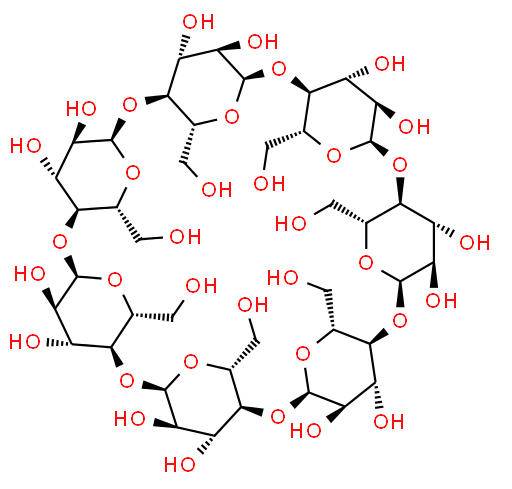
\includegraphics[width=\textwidth]{image24}
    \caption*{(b) β-ТД}
  \end{subfigure}
  \caption*{Сурет 2 -- Зерттеу нысандарының құрылымдарының формулалары}
\end{figure}

\begin{multicols}{2}
(ХД)-дың β-ТД-мен қосылу кешендері (1:1; 1:2; 1:3) сулы-спиртті ортада
алынды. ХД мен β-ТД (ммоль ) қоспасы 600 секунд ішінде "Anton Paar
monowave 300" микротолқынды пеште 200 Вт сәулелену қуатымен 70°С
температурада әр 2 минуттік қадаммен өңделінді. Өңдеу аяқталғаннан кейін
еріткіштер алынып тасталды, ал өнімдер ацетонмен жуылып, эксикатор
ішінде CaCl\textsubscript{2} көмегімен тұрақты массаға дейін кептірілді.
β-ТД:ХД клатрат кешендерінің шығысы келесідей болды: 52,2 (1:1), 64.3
(1:2), 63,1 (1:3)\%. Алынған кешендер суда еритін ақ түсті кристалды
заттар болды, олар суда ақшыл түсті коллоидты ерітінді түзді. β-ТД:ХД
(2:1) кешенінің тазартылған суда ерігіштігі 0,20 мг±0,05/100 мл құрады.
β-ТД:ХД клатрат үлгілерінің бетінің морфологиясы LMN (Чехия) фирмасының
TesconMira3 сканерлеуші электронды микроскопының (СЭМ) көмегімен
зерттелді. ИҚ спектрлері 4000-400 см\textsuperscript{-1} диапазонында
Agilent Technologies (АҚШ) фирмасының CARY600 сериялы ИҚ-Фурье
спектрометрінде түсірілді. Алынған клатраттардың \textsuperscript{1}Н
және \textsuperscript{13}С ЯМР спектрлері DMSO-d6 еріткішін пайдаланып
Jnm-ECA Jeol400 спектрометрінде (сәйкесінше 399,78 және 100,53 МГц
жиіліктерде) тіркелді. β-ТД:ХД клатрат кешендерінің жылулық қасиеттері
labsys Evalution DTA/DTS дифференциалды сканерлеу калориметрінде
динамикалық режимде 30-500\textsuperscript{о}С температура диапазонында
азот атмосферасында 10 градус/мин қыздыру кезінде
Al\textsubscript{2}O\textsubscript{3} табақшасында жүргізілді,
температура диапазоны 30-800°С, үлгілердің қыздыру жылдамдығы 5-тен 20
к/мин дейін, үлгілердің массасы 12-16 мг болды, барлық есептеулер
Mathcad бағдарламасының көмегімен жүргізілді {[}11{]}.

{\bfseries Нәтижелер және талқылау.} Молекулалық докинг әдісі тұрақты кешен
пайда болған кезде бір молекуланың екіншісіне қатысты артықшылықты
конфигурациясын дұрыс болжауға мүмкіндік береді. Сандық бағалау ретінде
рецептор молекуласы мен лиганд арасындағы байланыс энергиясы
қолданылады. Бастапқыда біз (β-ТД-дың β-ТД:ХД молекуласымен молекулалық
докингін олардың қосу кешендерінің 1:1 қатынасында байланысу энергиясын
анықтау үшін жасадық. (сурет 3).
\end{multicols}

\begin{figure}[H]
\centering
\begin{minipage}{0.4\textwidth}
\centering
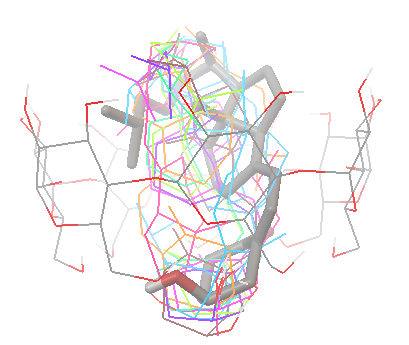
\includegraphics[width=\textwidth]{image25}
\end{minipage}
\hfill
\begin{minipage}{0.4\textwidth}
\centering
\begin{tabular}{|p{0.45\textwidth}|p{0.45\textwidth}|}
\hline
\textbf{Конформация нөмері} & \textbf{Байланыс энергиясы, ккал/моль} \\
\hline
4 & -2.70 \\
7 & -0.17 \\
10 & +1.70 \\
6 & +4.22 \\
3 & +7.45 \\
8 & +17.43 \\
1 & +17.68 \\
5 & +27.93 \\
9 & +8.98 \\
2 & +23.00 \\
\hline
\end{tabular}
\end{minipage}
\caption*{(а) ХД-нің β-ТД-нің іш қуысындағы 10 түрлі мүмкін конформациясы}
\end{figure}

\begin{figure}[H]
\centering
\begin{subfigure}[b]{0.4\textwidth}
\centering
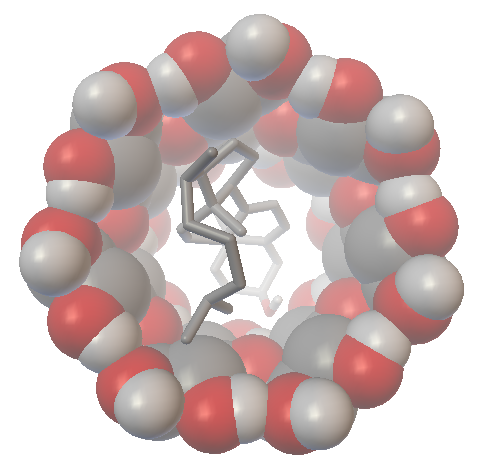
\includegraphics[width=\textwidth]{image26}
\caption*{Жоғарыдан көрініс}
\end{subfigure}
\hfill
\begin{subfigure}[b]{0.4\textwidth}
\centering
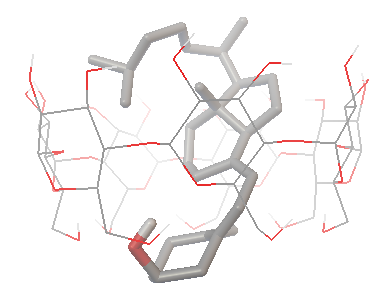
\includegraphics[width=\textwidth]{image27}
\caption*{Бүйірден көрініс}
\end{subfigure}
\caption*{(b) Ең жақсы байланысқан конформация (байланыс энергиясы = –2.7 ккал/моль)}
\caption*{Сурет 3 – Холекальциферолдың β-ТД-мен докинг нәтижелері}
\end{figure}

\begin{multicols}{2}
Докинг негізінде β-ТД мен ХД лигандысының 10 конформациясы алынды және
олардың байланысу энергиясы бағаланды. Сонымен қатар, ең жақсы
байланыстыруды 4-ші конформация көрсетті, оның байланысу энергиясы -2,7
ккал/моль болды. Байланыстыру энергиясының теріс мәні β-ТД-мен ХД
молекулалары арасында комплекс түзілуінінің мүмкіншілігін көрсетеді,
сонымен бірге өте төмен мән комплекс түзілу реакциясын жүргізудің арнайы
шарттарының қажеттілігі туралы айтуға мүмкіндік береді. ХД мен β-ТД
арасындағы байланыс энергиясының аз мөлшері назар аударады, сондықтан
AutoDock құралдарының көмегімен рецептор мен лиганд молекулалары
арасындағы сутегі байланыстарының болуын анықтау қызықты болып көрінді
(сурет 4).
\end{multicols}

\begin{figure}[H]
\centering
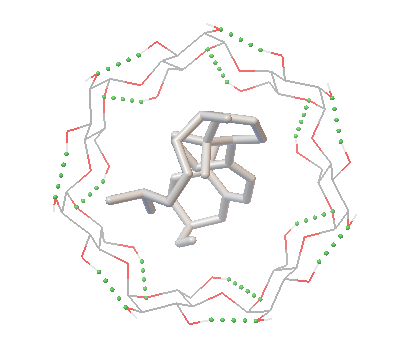
\includegraphics[width=0.4\textwidth]{image28}
\caption*{Сурет 4 -- ХД-дың β-ТД-мен кешендеріндегі}
\end{figure}

\begin{multicols}{2}
14 сутегі байланысының жүйесі

4-Суретте көрсетілген мәліметтерден бойынша β-ТД молекуласындағы ОН
топтары арасында 14 молекулаішілік сутегі байланысының жүйесі түзіледі.
Бұл жағдайда рецептор мен лиганд молекулалары арасында сутегі байланысы
байқалмайды. Рецептор мен лиганд арасында молекулааралық сутегі
байланысының болмауы олардың ТД-мен кешендерін молярлық 2:1 қатынасында
модельдеу болды. Ыңғайлы болу үшін β-ТД молекуласының кең жағы "бас"
("бас"), ал қарама-қарсы артқы жағы "құйрық" ("құйрық") деп белгіленді
(сурет. 5а). Бұл жағдайда екі β-ТД молекуласы арасында өзара
бағдарлаудың үш түрі болуы мүмкін: "бас-бас" (HH), бас-құйрық (HT) және
"құйрық-құйрық" (TT) (сурет 5б-г).
\end{multicols}

\begin{figure}[H]
\centering
\begin{subfigure}[b]{0.4\textwidth}
\centering
\caption*{«Бас» («Head»)}
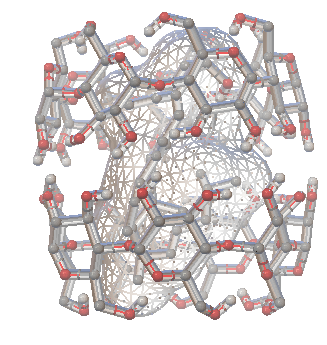
\includegraphics[width=\textwidth]{image29}
\caption*{«Құйрық» («Tail»)}
\caption*{(a) β-ТД молекуласының бас және құйрығы}
\end{subfigure}
\begin{subfigure}[b]{0.4\textwidth}
\centering
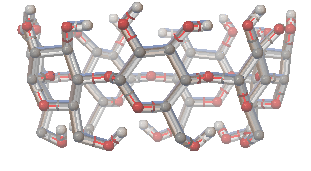
\includegraphics[width=\textwidth]{image30}
\caption*{(б) кешеннің «бас басқа» (НН) түрі \\
(байланыс энергиясы = -4.71 ккал/моль)}
\end{subfigure}
\begin{subfigure}[b]{0.4\textwidth}
\centering
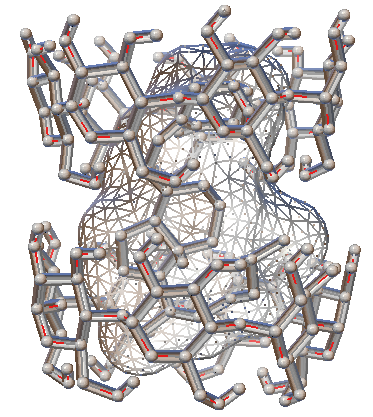
\includegraphics[width=\textwidth]{image31}
\caption*{(c) кешеннің «бас құйрыққа» түрі (HT), \\
(байланыс энергиясы = -7.32 ккал/моль)}
\end{subfigure}
\begin{subfigure}[b]{0.4\textwidth}
\centering
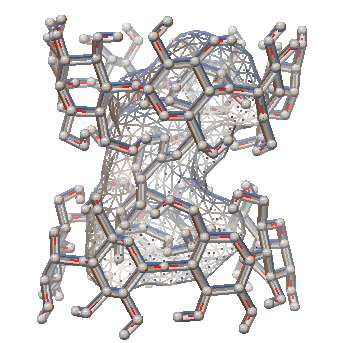
\includegraphics[width=\textwidth]{image32}
\caption*{(д) кешеннің «құйрық құйрыққа» түрі (TT), \\
(байланыс энергиясы = +3.85 ккал/моль)}
\end{subfigure}
\caption*{Сурет 5 -- β-ТД молекуласы (а) және оның ХД-мен кешендерінің үш түрі (2:1)}
\end{figure}

\begin{multicols}{2}
5-Суретте көрініп тұрғандай, 1:1 (-2,7 ккал/моль) комплексімен
салыстырғанда, "бас-бас" (HH) және "бас-құйрық" (HT) кешендерінің екі
түрі тиімдірек байланыстыруды (тиісінше -4,71 және -7,32 ккал/моль)
көрсетеді. "Құйрық-құйрық" типті кешен оң байланыс энергиясын көрсетеді,
бұл осы типтегі кешеннің түзілу мүмкіншілігінің аз екенін көрсетеді. Бұл
жағдайда "бас-құйрық" (с) кешені максималды байланыс энергиясын
көрсетеді, бұл мұндай кешеннің үлкен тұрақтылығын көрсетеді {[}11,12{]}.

Қарастырылып отырған физикалық жағдайға байланысты зерттелетін
объектілерді сипаттау үшін әртүрлі әдістерді қолдану модельдердің
сенімділігі тұрғысынан жақсы нәтиже береді. 6-Суретте β-ТД-нің, β-ТД+ ХД
физикалық қоспасының және β-ТД:ХД (2:1) қосылу кешенінің микросуреттері
көрсетілген. Клатрат түзілуіндегі кристалл беті морфологиясының өзгеруі
қосу кешенінің пайда болуының күшті дәлелі болып табылады {[}13,14{]}.
\end{multicols}

\begin{figure}[H]
\centering
\begin{subfigure}[b]{0.3\textwidth}
\centering
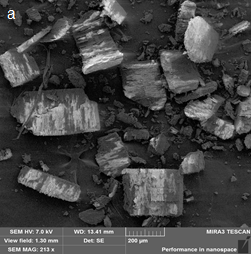
\includegraphics[width=\textwidth,height=\textwidth]{image33}
\end{subfigure}
\begin{subfigure}[b]{0.3\textwidth}
\centering
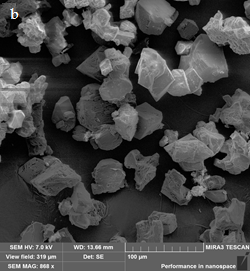
\includegraphics[width=\textwidth,height=\textwidth]{image34}
\end{subfigure}
\begin{subfigure}[b]{0.3\textwidth}
\centering
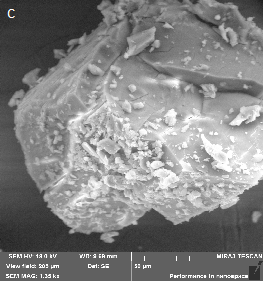
\includegraphics[width=\textwidth,height=\textwidth]{image35}
\end{subfigure}
\begin{subfigure}[b]{0.3\textwidth}
\centering
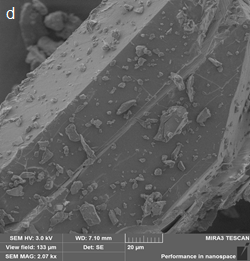
\includegraphics[width=\textwidth,height=\textwidth]{image36}
\end{subfigure}
\begin{subfigure}[b]{0.3\textwidth}
\centering
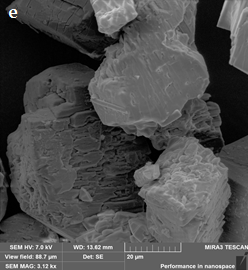
\includegraphics[width=\textwidth,height=\textwidth]{image37}
\end{subfigure}
\begin{subfigure}[b]{0.3\textwidth}
\centering
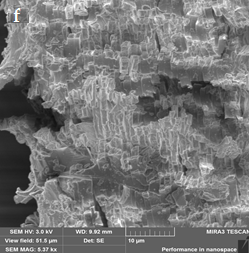
\includegraphics[width=\textwidth,height=\textwidth]{image38}
\end{subfigure}
\caption*{Сурет 6 -- β-ТД (а, b), β-ТД +ХД-ның физикалық қоспасының және β-ТД:ХД (2:1) (e, f) \\
клатратының әр түрлі үлкейтудегі электронды микросуреттері}
\end{figure}

\begin{multicols}{2}
ИҚ спектрлерде (сурет 7) О-Н байланысының валенттік тербелістері 3398
(β-ТД (a), 3564 (ТД\textsubscript{3} (b) және 3368
см\textsuperscript{--1} (β-ТД:ХД (c) аймақтарында кең жолақ түрінде
анықталады. Сондай-ақ, CH және CН\textsubscript{2} топтарындағы CH
байланыстарының валенттік тербелістеріне тән сіңіру жолағы 2924
см\textsuperscript{-1}-де бар {[}15{]}. β-ТД:ХД кешенінің ИҚ
спектрлерінде C=C, ОН және ВД\textsubscript{3}-ның басқа топтарының
сіңіру жолақтары көрінбейді. Бұл осы топтардың толқын ұзындығының бірдей
диапазонында өте кең және қарқынды β-ТД жолақтарының көлеңкесінен
көрінбеуі мүмкін. 1643 см\textsuperscript{-1} аймағында β-ТД:ХД
кешенінің С=О тобының қарқынды жолағы бар. Қосылу кешендерінің түзілуін
растаудың ақпараттық әдістерінің бірі-спектроскопияның
\textsuperscript{1}Н ЯМР әдісі {[}16{]}. Бұл әдіс ТД молекуласының ішкі
қуысында бағытталған β-ТД H-3 және H-5 протондарының тербелмелі
спектрлеріндегі олардың химиялық ыдысуын айқын байқауға мүмкіндік
береді. Клатраттың \textsuperscript{1}Н ЯМР спектрінде барлық алты β-ТД
протондары күшті өрісте айқын химиялық ыдысуды көрсетті. β-ТД:ХД (2:1)
кешенінің \textsuperscript{1}H ЯМР спектрлеріндегі Δδ химиялық ыдысу
мәндеріндегі ең үлкен айырмашылық H-3 (-0.112) және H-5 (-0.108)
сфераішілік протондарына тән. Бұл деректер циклодекстриннің гидрофобты
қуысында ішкі (инклюзивті) кешен пайда болады деген қорытынды жасауға
мүмкіндік береді.
\end{multicols}

\begin{figure}[H]
\centering
\begin{subfigure}[b]{0.45\textwidth}
\centering
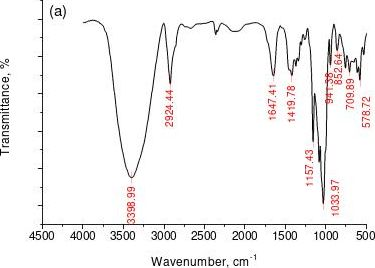
\includegraphics[width=\textwidth]{image39}
\end{subfigure}
\begin{subfigure}[b]{0.45\textwidth}
\centering
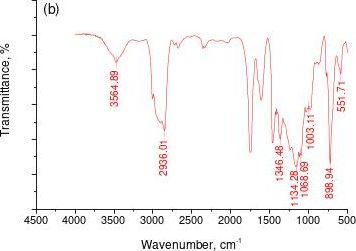
\includegraphics[width=\textwidth]{image40}
\end{subfigure}
\begin{subfigure}[b]{0.45\textwidth}
\centering
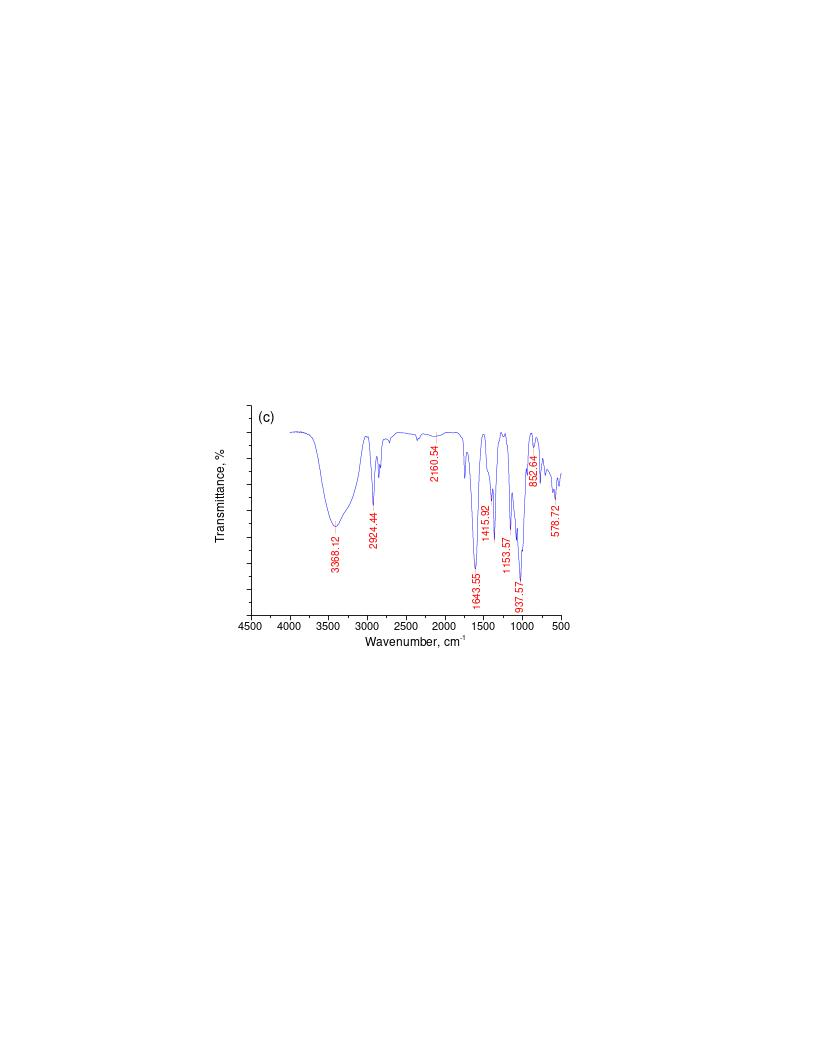
\includegraphics[width=\textwidth]{image41}
\end{subfigure}
\caption*{Сурет 7 -- β-ТД (a), ХД (b) және β-ТД:ХД (2:1) клатратының ИК спектрлері}
\end{figure}

\begin{multicols}{2}
β-ТД:ДД\textsubscript{3} кешендерінің термиялық қасиеттерін талдау
термогравиметриялық талдау әдісімен жүргізілді {[}17{]}. Суретте 8а,b
β-ТД мен оның β-ТД:ХД (2:1) клатратының ТГ мен ДТГ термограммалары
көрсетілген (қыздыру жылдамдығы 10 градус/мин).

β-ТД және оның β-ТД:ХД клатратының термоаналитикалық ыдырау
көрсеткіштері (2:1) TГ/ДTГ сызықтық қисықтарымен ұсынылған (сурет 8a,b).
Термогравиметриялық β-ТД қисықтары мен β-ТД:ХД клатратын салыстыру
арқылы (сурет 8a,b), β-ТД:ХД клатраты үшін
\textasciitilde124\textsuperscript{о}\textasciitilde{} \textasciitilde{}
235\textsuperscript{о}С температура диапазонында үлгі массасының
қарқынды төмендеуі байқалатынын көреміз (\textasciitilde77,27 \%). TG
қисығының бұл бөлімі \textasciitilde235\textsuperscript{о}С
температурада ДТГ қисығындағы массаның жоғалу жылдамдығының максималды
өзгеруіне сәйкес келеді (сурет 8b).
\end{multicols}

\begin{figure}[H]
\centering
\begin{subfigure}[b]{0.8\textwidth}
\centering
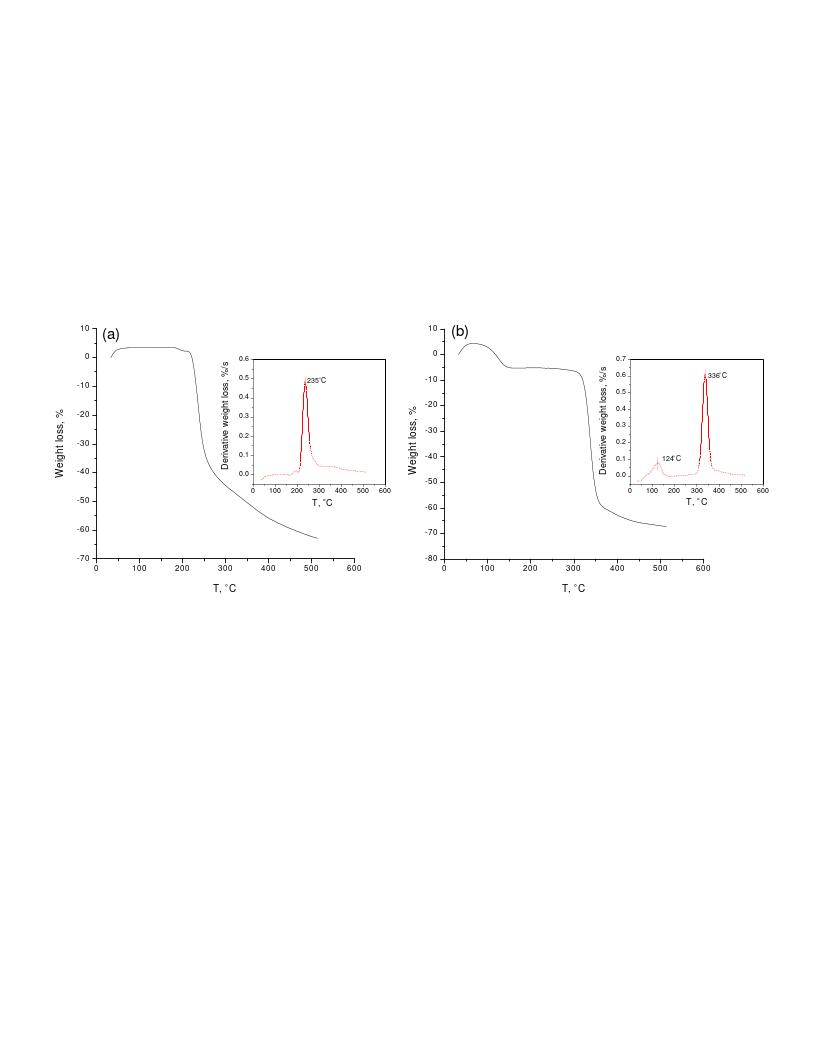
\includegraphics[width=\textwidth]{image42}
\end{subfigure}
\caption*{Сурет 8 -- β-ТД:ХД кешенінің азотты ортада 10 градус/мин тұрақты қыздыру
жылдамдығы жағдайында алынған TГ/ДТГ қисықтары: а) физикалық қоспа; b)
β-ТД:ХД (2:1)}
\end{figure}


\begin{multicols}{2}
β-ТД:ХД клатраттарындағы массаның төмен температурада
(\textasciitilde1240с) жоғалуы ылғалдың жойылуымен байланысты, бұл ДТГ
деректерімен де расталады (сурет 8b). Алынған β-ТД:ХД кешендерінде,
бастапқы β-ТД сияқты, байланысқан су болды. Алынған мәліметтер негізінде
β-ТД:ХД (2:1) клатратының термиялық ыдырауының кинетикалық параметрлері
есептелді (кесте 3) {[}13{]}. β-ЦД мен β-ТД:ХД (2:1) клатратының
термиялық тұрақтылығын салыстыру үшін ыдырау реакциясының активтену
энергиялары анықталды. β-ЦД және β-ТД:ХД (2:1) кешендерінің термиялық
ыдырауының есептеулерін салыстыра отырып β-ТД мен оның клатратының (2:1)
активтену энергиялары бірдей конверсия дәрежелерінде (\emph{α}) әр түрлі
болады деп айтуға болады (кесте).
\end{multicols}

\begin{longtable}[]{@{}
  >{\raggedright\arraybackslash}p{(\columnwidth - 4\tabcolsep) * \real{0.3037}}
  >{\raggedright\arraybackslash}p{(\columnwidth - 4\tabcolsep) * \real{0.3750}}
  >{\raggedright\arraybackslash}p{(\columnwidth - 4\tabcolsep) * \real{0.3212}}@{}}
\caption*{Кесте -- β-ТД мен β-ТД:ХД (2:1) клатратының азотты ортада активтену
энергиясының мәндері} \\
\toprule\noalign{}
\begin{minipage}[b]{\linewidth}\raggedright
Үлгі
\end{minipage} & \begin{minipage}[b]{\linewidth}\raggedright
E\textsubscript{a}, кДж/моль
\end{minipage} & \begin{minipage}[b]{\linewidth}\raggedright
A, с\textsuperscript{-1}
\end{minipage} \\
\midrule\noalign{}
\endhead
\bottomrule\noalign{}
\endlastfoot
β-ТД & 164.58 & 1.10·10\textsuperscript{17} \\
β-ТД:ХД (2:1) & 103.50 & 8.96·10\textsuperscript{10} \\
\end{longtable}

\begin{multicols}{2}
{\bfseries Қорытынды.} Жүргізілген зерттеулердің нәтижелері
холекальциферолдың (ХД) β-олигоқантпен (β-ТД) суда еритінді қосылу
кешенін алу мүмкіндігін көрсетті, оны тағамды дәрумендеу үшін қолдануға
болады. \emph{In silico} зерттеу жағдайында молекулалық модельдеу және
докинг әдістерін қолдану ХД-нің β-ТД-мен қосылу кешендерінің түзілу
механизмдерінің жалпы көрінісін жасауға мүмкіндік берді. Модельдер
жартылай иілгіш қондыру әдісін қолданды, онда рецептор қатты зат ретінде
қарастырылды, ал лиганд белгілі бір текше аймақта айналды және қозғалыс
жағдайында болды. Зерттелетін объектілерді сипаттау үшін қарастырылып
отырған физикалық жағдайға байланысты әртүрлі физиохимиялық әдістерді
қолдану модельдердің сенімділігі тұрғысынан жақсы нәтиже береді. Майлы
ортада еритін ХД дәруменінің β-олигоқантпен микротолқынды белсендіру
жағдайында сулы-спиртті ортада әрекеттесуі оның суда еритін
супрамолекулярлы қосылу кешенінің түзілуіне әкелді. ХД-ді клатратты
кешенге қаптау дәруменнің майлы ерітіндісінің агрегаттық күйінің
өзгеруіне әкелді. Синтезделген β-ТД:ХД кешені "қонақ-қожайын"
қосылыстарына жатады және жақсы ерігіштікке ие. Клатрат кешенінің
түзілуіндегі шешуші мәселе арнайы байланыс емес (гидрофобты,
дисперсиялық және ван-дер-Ваальс) өзара әрекеттесулерге жатады.
\end{multicols}

\emph{Алғыс, мүдделер қақтығысы (қаржыландыру{\bfseries )-} Қаржыландыру,
биологиялық белсенді заттарды инкапсуляциялау әдістерін әзірлеу
жөніндегі ғылыми зерттеуді Қазақстан Республикасы Білім және ғылым
министрлігінің Ғылым комитеті қолдады (PTF № BR10965230, 2021-2023).}

{\bfseries Әдебиеттер}

\begin{enumerate}
\item
Mauryaa V.K., Bashirb K., Aggarwala M. Vitamin D microencapsulation
and fortification: Trends and technologies // Journal of Steroid
Biochemistry and Molecular Biology. --2020. --Vol.196. --No.105489.

\item
Brett N.R., Lavery P., Vanstone C.A., Maguire J.L., Rauch F., Weiler
H.A. Dietary vitamin D dose-response in healthy children 2 and 8 y of
age: a 12-wk randomized controlled trial using fortified foods // Am. J.
Clin. Nutr. --2016. -- Vol. 103. --P.144-152.

\item
Abu el Maaty M., Almouhanna F., Wölfl S. Expression of TXNIP in
cancer cells and regulation by 1, 25 (OH) 2D\textsubscript{3}: is it
really the vitamin D\textsubscript{3} upregulated protein // Int. J.
Mol. Sci. --2018. --Vol.19. -- Issue No 3. --P.796-803.

\item
Atteritano M., Mirarchi L., Venanzi-Rullo E., Santoro D., Iaria C.,
Catalano A., Lasco A., Arcoraci V., Lo Gullo A., Bitto A. Vitamin D
status and the relationship with bone fragility fractures in
HIV-infected patients: a case control study // Int. J. Mol. Sci. --2018.
--Vol.19. --P.119.

\item
Legarth C., Grimm D., Wehland M., Bauer J., Krüger M. The impact of
vitamin D in the treatment of essential hypertension. Int. J. Mol. Sci.
--2018. --Vol.19. --Issue No 2. --P. 455.

\item
Wierzbicka J., Binek A., Ahrends T., Nowacka J.D., Szydłowska A.,
Tuckey R. Differential antitumor effects of vitamin D analogues on
colorectal carcinoma in culture // Int. J. Oncol. --2015. --Vol. 47.
--P.1084-1096.

\item
Larsen, K.L. Large cyclodextrins //J. Incl. Phenom. Mycrocycl. Chem.
--2002, -- Vol.43(1), --Р.1-13.

\item
Zhao D., Liao K., Ma X., Yan X. Study of the supramolecular inclusion
of~\emph{β}-cyclodextrin with andrographolide //
\href{https://link.springer.com/journal/10847}{Journal of Inclusion
Phenomena and Macrocyclic Chemistry}. --2002. --Vol.43. --259-264.

9 Morris G. M., Huey R., Lindstrom W., Sanner M. F., Belew R. K.,
Goodsell D.S. and Olson A.J. ``Autodock4 and AutoDockTools4: automated
docking with selective receptor flexibility // J. Computational
Chemistry. --2009. --Vol.16. --P.2785-2791.

\item
Fuhrmann J., Rurainski A., Lenhof H. P., Neumann D. A new Lamarckian
genetic algorithm for flexible ligand-receptor docking // Journal of
computational chemistry. --2010. --Vol. 31. -- Issue No.9.
--P.1911--1918.

\item
Kim S., Chen J., Cheng T., Gindulyte A., He J., He S., Li Q.,
Shoemaker B. A., Thiessen P.A., Yu B., Zaslavsky L., Zhang J.,
\emph{Bolton E.E.} PubChem in 2021: new data content and improved web
interfaces \emph{//~}Nucleic Acids Res.~ --2019. --Vol.49(D1).
--P.D1388--D1395.

\item
Bulani V.D., Kothavade P.S., Kundaikar H.S., Gawali N.B., Chowdhury
A.A., Degani M.S., Juvekar A.R. Inclusion complex of ellagic acid with
β-cyclodextrin: Characterization and in vitro anti-inflammatory
evaluation //~J. Mol. Struct\emph{.}~--2016. --Vol.1105. --P.308-315.

\item
Bakirova R., Nukhuly A., Iskineyeva A., Fazylov S., Burkeev M.,
Mustafaeva A., Minaeva E., Sarsenbekova A. Obtaining and Investigation
of the beta-Cyclodextrin Inclution Complex with Vitamin
D\textsubscript{3} Oil // Scientifica. --2020. --Vol.1-8. ~-- ID
6148939. DOI: 10.1155/2020/6148939.

\item
Liu Y., Zhang H. ``Study of VD\textsubscript{3}-β-Cyclodextrin
Inclusion Complex //Journal of Geoscience and Environment
Protection\emph{.} --2016. --Vol.4. --Issue 4. --P.163-167

\item
Zou A., Zhao X., Handge U.A., Garamus V.M., Willumeit-Römer R., Yin
P. Folate receptor targeted bufalin/\emph{β}-cyclodextrin supramolecular
inclusion complex for enhanced solubility and anti-tumor efficiency of
bufalin //Mater. Sci. Eng. --2017. --Vol.78. --P.609-618.

\item
Dodziuk H., Koźmiński W., Ejchart A. NMR studies of chiral
recognition by cyclodextrines //Chirality\emph{.} --2004. -- Vol.16.
--Issue No.2. --P.90-105.
\end{enumerate}

{\bfseries References}


\begin{enumerate}
\item
Mauryaa V.K., Bashirb K., Aggarwala M. Vitamin D microencapsulation
and fortification: Trends and technologies // Journal of Steroid
Biochemistry and Molecular Biology. --2020. --Vol.196. --No.105489.

\item
Brett N.R., Lavery P., Vanstone C.A., Maguire J.L., Rauch F., Weiler
H.A. Dietary vitamin D dose-response in healthy children 2 and 8 y of
age: a 12-wk randomized controlled trial using fortified foods // Am. J.
Clin. Nutr. --2016. -- Vol. 103. --P.144-152.

\item
Abu el Maaty M., Almouhanna F., Wölfl S. Expression of TXNIP in
cancer cells and regulation by 1, 25 (OH) 2D\textsubscript{3}: is it
really the vitamin D\textsubscript{3} upregulated protein // Int. J.
Mol. Sci. --2018. --Vol.19. -- Issue No 3. --P.796-803.

\item
Atteritano M., Mirarchi L., Venanzi-Rullo E., Santoro D., Iaria C.,
Catalano A., Lasco A., Arcoraci V., Lo Gullo A., Bitto A. Vitamin D
status and the relationship with bone fragility fractures in
HIV-infected patients: a case control study // Int. J. Mol. Sci. --2018.
--Vol.19. --P.119.

\item
Legarth C., Grimm D., Wehland M., Bauer J., Krüger M. The impact of
vitamin D in the treatment of essential hypertension. Int. J. Mol. Sci.
--2018. --Vol.19. --Issue No 2. --P. 455.

\item
Wierzbicka J., Binek A., Ahrends T., Nowacka J.D., Szydłowska A.,
Tuckey R. Differential antitumor effects of vitamin D analogues on
colorectal carcinoma in culture // Int. J. Oncol. --2015. --Vol. 47.
--P.1084-1096.

\item
Larsen, K.L. Large cyclodextrins //J. Incl. Phenom. Mycrocycl. Chem.
--2002, -- Vol.43(1), --Р.1-13.

\item
Zhao D., Liao K., Ma X., Yan X. Study of the supramolecular inclusion
of~\emph{β}-cyclodextrin with andrographolide //
\href{https://link.springer.com/journal/10847}{Journal of Inclusion
Phenomena and Macrocyclic Chemistry}. --2002. --Vol.43. --259-264.

\item
Morris G. M., Huey R., Lindstrom W., Sanner M. F., Belew R. K.,
Goodsell D.S. and Olson A.J. ``Autodock4 and AutoDockTools4: automated
docking with selective receptor flexibility // J. Computational
Chemistry. --2009. --Vol.16. --P.2785-2791.

\item
Fuhrmann J., Rurainski A., Lenhof H. P., Neumann D. A new Lamarckian
genetic algorithm for flexible ligand-receptor docking // Journal of
computational chemistry. --2010. --Vol. 31. -- Issue No.9.
--P.1911--1918.

\item
Kim S., Chen J., Cheng T., Gindulyte A., He J., He S., Li Q.,
Shoemaker B. A., Thiessen P.A., Yu B., Zaslavsky L., Zhang J.,
\emph{Bolton E.E.} PubChem in 2021: new data content and improved web
interfaces \emph{//~}Nucleic Acids Res.~ --2019. --Vol.49(D1).
--P.D1388--D1395.

\item
Bulani V.D., Kothavade P.S., Kundaikar H.S., Gawali N.B., Chowdhury
A.A., Degani M.S., Juvekar A.R. Inclusion complex of ellagic acid with
β-cyclodextrin: Characterization and in vitro anti-inflammatory
evaluation //~J. Mol. Struct\emph{.}~--2016. --Vol.1105. --P.308-315.

\item
Bakirova R., Nukhuly A., Iskineyeva A., Fazylov S., Burkeev M.,
Mustafaeva A., Minaeva E., Sarsenbekova A. Obtaining and Investigation
of the beta-Cyclodextrin Inclution Complex with Vitamin
D\textsubscript{3} Oil // Scientifica. --2020. --Vol.1-8. ~-- ID
6148939. DOI: 10.1155/2020/6148939.

\item
Liu Y., Zhang H. ``Study of VD\textsubscript{3}-β-Cyclodextrin
Inclusion Complex //Journal of Geoscience and Environment
Protection\emph{.} --2016. --Vol.4. --Issue 4. --P.163-167

\item
Zou A., Zhao X., Handge U.A., Garamus V.M., Willumeit-Römer R., Yin
P. Folate receptor targeted bufalin/\emph{β}-cyclodextrin supramolecular
inclusion complex for enhanced solubility and anti-tumor efficiency of
bufalin //Mater. Sci. Eng. --2017. --Vol.78. --P.609-618.

\item
Dodziuk H., Koźmiński W., Ejchart A. NMR studies of chiral
recognition by cyclodextrines //Chirality\emph{.} --2004. -- Vol.16.
--Issue No.2. --P.90-105.
\end{enumerate}

\emph{{\bfseries Information about authors:}}

\begin{itemize}
\item
Serik Fazylov -- Academician of the National Academy of the Republic of
Kazakhstan, Doctor of Chemical Sciences, Full Professor, Institute of
Organic Synthesis and Coal Chemistry, Alikhanov str. 1, 100008,
Karaganda, Kazakhstan; е-mail:
\url{iosu8990@mail.ru};
\url{https://orcid.org/0000-0002-4240-6450}. \emph{(Corresponding
author)}

\item
Oralgazy Nurkenov -- Doctor of Chemical Sciences, Full Professor,
Institute of Organic Synthesis and Coal Chemistry, Alikhanov str. 1,
100008, Karaganda, Kazakhstan; е-mail:
\href{mailto:nurkenov_oral@mail.ru}{nurkenov\_oral@mail.ru};
\url{https://orcid.org/0000-0003-1878-2787}.

\item
Ainara Iskineyeva - PhD student of Saken Seifullin Kazakh Agrotechnical
University, Nur-Sultan, Kazakhstan, e-mail: iskeneeva\_aynara@mail.ru,
https://orcid.org/0000-0002-1705-6372.

\item
Ayaulim Mustafayeva - Candidate of Thechnical Sciences, Saken Seifullin
Kazakh Agrotechnical University, Nur-Sultan, Kazakhstan, e-mail:
ayaulym.mustafa@mail.ru,
\href{https://orcid.org/0000-0003-0693-6427}{https://orcid.org/0000-0003-0693-6427}.

\item
Irina Pustolaikina -- Candidate of Chemical Sciences, Assoc. Professor,
Karagandy University of the name of academician E.A.~Buketov,
Universitetskaya street, 28, 100024, Karaganda, Kazakhstan; e-mail:
\href{mailto:ipustolaikina@gmail.com}{ipustolaikina@gmail.com},
\url{https://orcid.org/0000-0001-6319-666X}.

\item
Akmaral Sarsenbekova - PhD, Assoc. Professor,, Karagandy University of
the name of academician E.A.~Buketov, Universitetskaya street, 28,
100024, Karaganda, Kazakhstan; e-mail:
\href{mailto:chem_akmaral@mail.ru}{chem\_akmaral@mail.ru},
\url{https://orcid.org/0000-0002-8951-3616}.

\item
Aleksandr Sviderskiy -- Doctor of Chemical Sciences, Full Professor,
Innovativ Eurasian University, Lomova Str. 45, 140000, Pavlodar,
Kazakhstan; e-mail:
\href{mailto:katsostud@mail.ru}{katsostud@mail.ru},
https://orcid.org/0000-0001-7277-5882.
\end{itemize}
